\documentclass{beamer}


% Beamer Settings
\mode<presentation>
\usetheme{CambridgeUS}
\usecolortheme{beaver}
\setbeamerfont{footnote}{size=\tiny}

\usepackage{chemfig}
\usepackage{float}

\usepackage{multirow}
\usepackage{url}
\usepackage{framed}
\usepackage{graphicx}
\usepackage{enumerate}
\usepackage{threeparttable}
\usepackage{booktabs}
\usepackage{hyperref}
\usepackage{hyperxmp}
\usepackage{minipage-marginpar}
\usepackage{subfigure}
\usepackage{wrapfig}

%\usepackage{setspace}
\graphicspath{{fig/}}

% 让chemfig用无衬线字体
\renewcommand * \printatom[1]{\ensuremath{\mathsf{#1}}}

% Version Control
\newcommand{\thisversion}{v0.33}


% Changing Fonts to Arial
%\usefonttheme{professionalfonts} % using non standard fonts for beamer
%\usefonttheme{serif} % default family is serif
%\usepackage{fontspec}
%\setmainfont{Arial}

\hypersetup{pdfinfo={
		Author = {Jian-Qing Qi},
		Title = {Organoboron Compounds: Prevalent and Novel Applications},
		Keywords = {organoboron},
		Subject = {\thisversion} ,},
	pdfcopyright = {Copyright (C) 2019 by Jian-Qing Qi. All rights reserved.},
	pdflicenseurl = {https://alexander-qi.github.io/}}

\title[Organoboron]{Organoboron Compounds:\\ Prevalent and Novel Applications}

\author{Jian-Qing Qi}
\date{2019.12.3}
\institute{Tsinghua University}

%\logo{
\includegraphics[height=1cm]{tsinghua-logo.eps}}
\titlegraphic{
\includegraphics[height=1.5cm]{tsinghua-logo.eps}}


\usepackage[backend=bibtex,style=numeric,sorting=none]{biblatex}
\addbibresource{data/boron.bib} %BibTeX数据文件及位置
%\setbeamerfont{footnote}{size=\tiny}

\begin{document}
	\begin{frame}
	\titlepage
	
\end{frame}

\begin{frame}
\frametitle{Contents}
\tableofcontents
\end{frame}


\section{Introduction}

\begin{frame}
	\frametitle{Characteristics of Boron\footfullcite{RN3}}
	\begin{minipage}{\linewidth}
		
	
	\begin{minipage}[t]{0.45\linewidth}
		\begin{table}
		\caption{Atomic Radii}
		\begin{tabular}{ccc}
			\toprule
			&B&C\\
			\midrule
			$r_{vdw}$(\AA)&&1.70\\
			$r_{cov}$(\AA)&0.83&0.68\\
			\bottomrule
		\end{tabular}
	\end{table}	
	\end{minipage}
\hspace{0.05\linewidth}
\begin{minipage}[t]{0.45\linewidth}
	\begin{table}
		\caption{Bond Dissociation Energy}
		\begin{tabular}{cl}
			\toprule
			Bonds&$D_{298K}^{^\circ} \ (kJ \cdot mol^{-1})$\\
			\midrule
			\chemfig{B-[,0.5]B}&290\\
			\chemfig{B-[,0.5]H}&$345.2\pm 2.5$\\
			\chemfig{C-[,0.5]C}&$618\pm 15.4$\\
			\chemfig{C-[,0.5]H}&$318.4\pm 1.2$\\
					\chemfig{B-[,0.5]C}&$448\pm 29$\\
			\bottomrule
		\end{tabular}
	\end{table}
\end{minipage}
\end{minipage}
\end{frame}

\begin{frame}
\frametitle{Asymmetric Reduction of \chemfig{C=[,0.6]C}\footfullcite{RN7} and \chemfig{C=[,0.6]O}\footfullcite{RN6} Bonds}
%\setchemfig{fixed length=true}
%\schemestart[0,1.4] \chemname{\chemfig{IPC_2BH}}{99.1\% ee}\arrow{->[\chemfig{-[:30,0.4]=[:330,0.4]-[:30,0.4]}][248 K / 4.5 h]}{\chemfig{{IPC_2B}>[:30,0.6](-[2,0.6]-[:30,0.6])(-[:330,0.6])}}\arrow{->[[O]]}\chemname{\chemfig{{IPC_2B}>[:30,0.6](-[2,0.6]-[:30,0.6])(-[:330,0.6])}}{98.1\% ee} \schemestop
\begin{figure}
	\centering
	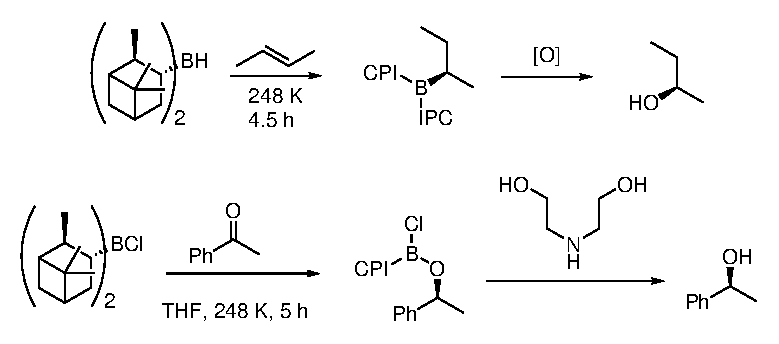
\includegraphics[width=0.9\linewidth]{fig/AsymmetricReduction}
	%\caption{Asymmetric Reduction of \chemfig{C=[,0.6]C} and \chemfig{C=[,0.6]O}}
	\label{fig:asymmetricreduction}
\end{figure}

\end{frame}

\begin{frame}
\frametitle{Diastereoselective Allylboration\footfullcite{RN4}}
\begin{figure}
	\centering
	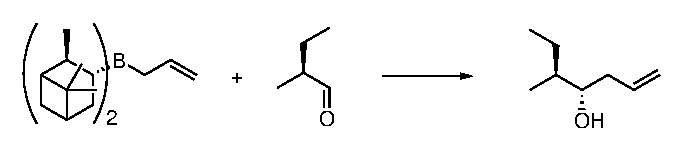
\includegraphics[width=0.8\linewidth]{fig/diastereo}
	\caption{Diastereoselective Allylboration}
	\label{fig:diastereo}
\end{figure}

\end{frame}

\begin{frame}
	\frametitle{Suzuki-Miyaura Cross-Coupling}
	\begin{figure}
		\centering
		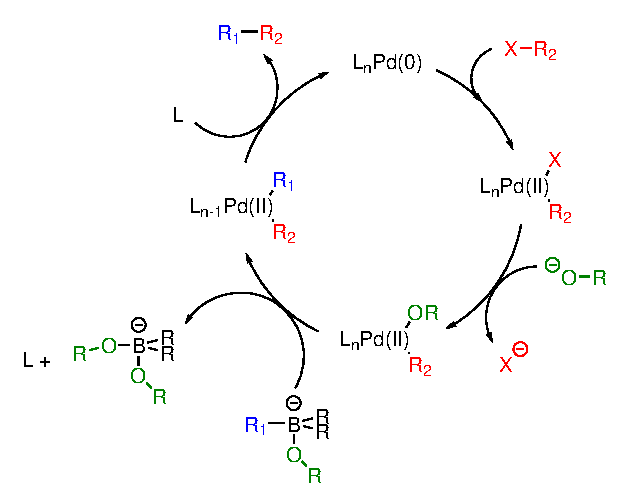
\includegraphics[width=0.7\linewidth]{fig/suzuki-miyaura}
		%\caption{}
		\label{fig:suzuki-miyaura}
	\end{figure}
	
\end{frame}

\section{Boron-Substituted 1,3-Dienes}

\begin{frame}
	\frametitle{Tandem Diels-Alder Cycloaddition}
	\begin{figure}
		\centering
		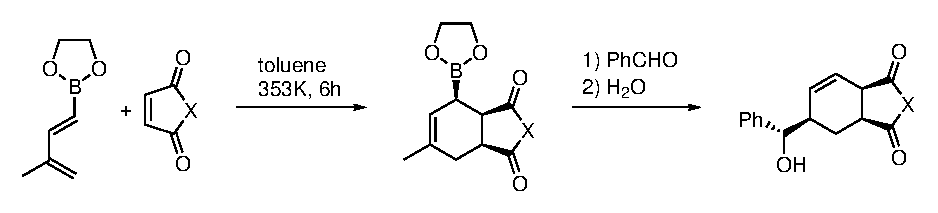
\includegraphics[width=1.0\linewidth]{fig/tand-diels-module}
		\caption{A Module Figure}
		\label{fig:tand-diels-module}
	\end{figure}
	
	
	The diastereoselectivity of this two-step process is
	very high, that is why this process is very important for generating
	multiple stereocentres from rather simple starting materials.\footfullcite{RN8}
	
\end{frame}

\begin{frame}
	\frametitle{A Synthetic Example\footfullcite{cannillo2013fast}}
	\begin{figure}
		\centering
		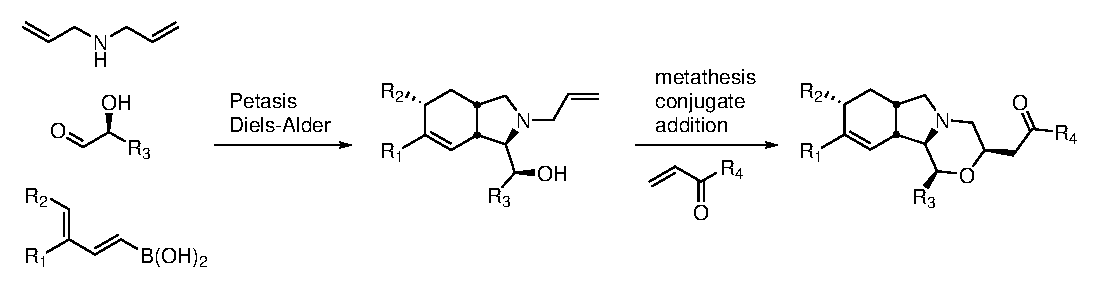
\includegraphics[width=1.0\linewidth]{fig/tand-diels-example}
		\caption{}
		\label{fig:tand-diels-example}
	\end{figure}
	
\end{frame}

\section{Organoboron Compounds for SET}

\begin{frame}
	\frametitle{Latest application of \chemfig{B_2 pin_2}\footfullcite{RN9}}
	\begin{figure}
		\centering
		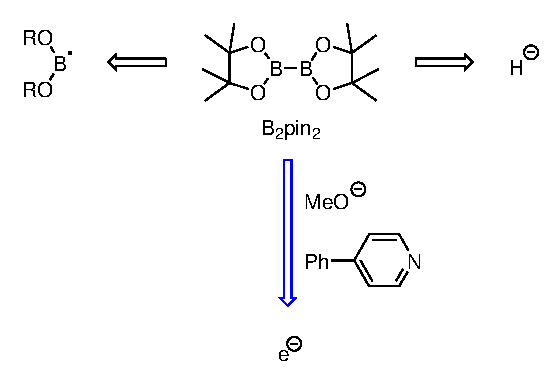
\includegraphics[width=0.8\linewidth]{fig/b2pin2-intro}
		\label{fig:b2pin2-intro}
	\end{figure}
	
\end{frame}

\begin{frame}
	\frametitle{Synthetic Applications of the New Method}
	When applied with \chemfig{B_2 pin_2}, p-PhPy, MeOK, the following reactions can take place\footfullcite{Pyridine}:
	\begin{figure}
		\centering
		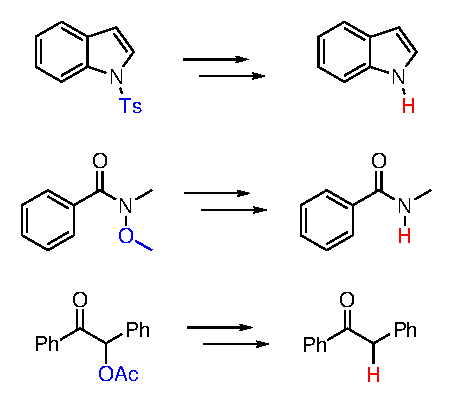
\includegraphics[width=0.44\linewidth]{fig/b2pin2-showcase}
		\label{fig:b2pin2-showcase}
	\end{figure}
	
\end{frame}

\begin{frame}
	\frametitle{Mechanisms of this Method}
	\begin{figure}
		\centering
		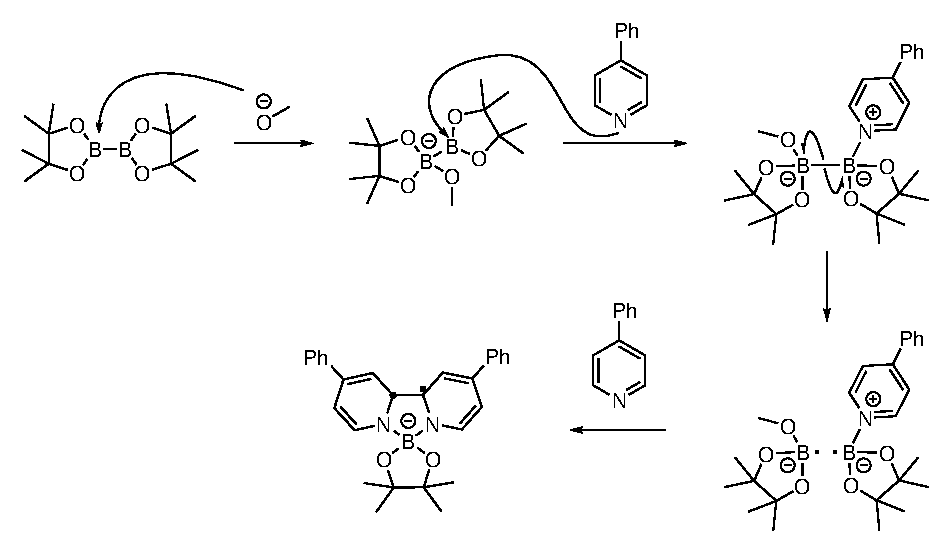
\includegraphics[width=0.8\linewidth]{fig/b2pin2mech}
		%\caption{}
		\label{fig:b2pin2mech}
	\end{figure}
	
\end{frame}

\section{Metal-Free Borylation}

\begin{frame}
	\frametitle{Metal-Free Directed \chemfig{C-[,0.6]H} Borylation\footfullcite{RN11}}
	\begin{figure}
		\centering
		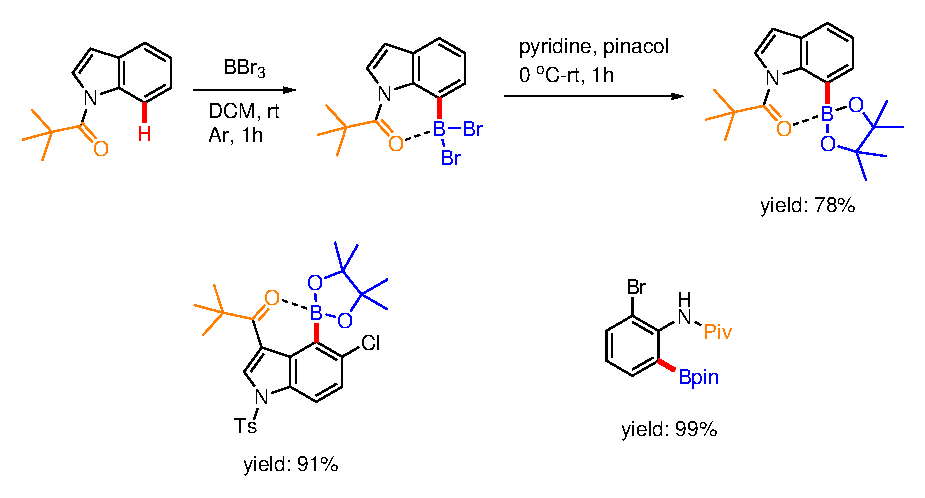
\includegraphics[width=0.9\linewidth]{metalfree}
		%\caption{}
		\label{fig:metalfree}
	\end{figure}
	
\end{frame}

\begin{frame}
	\frametitle{Mechanism of this Reaction}
	\begin{figure}
		\centering
		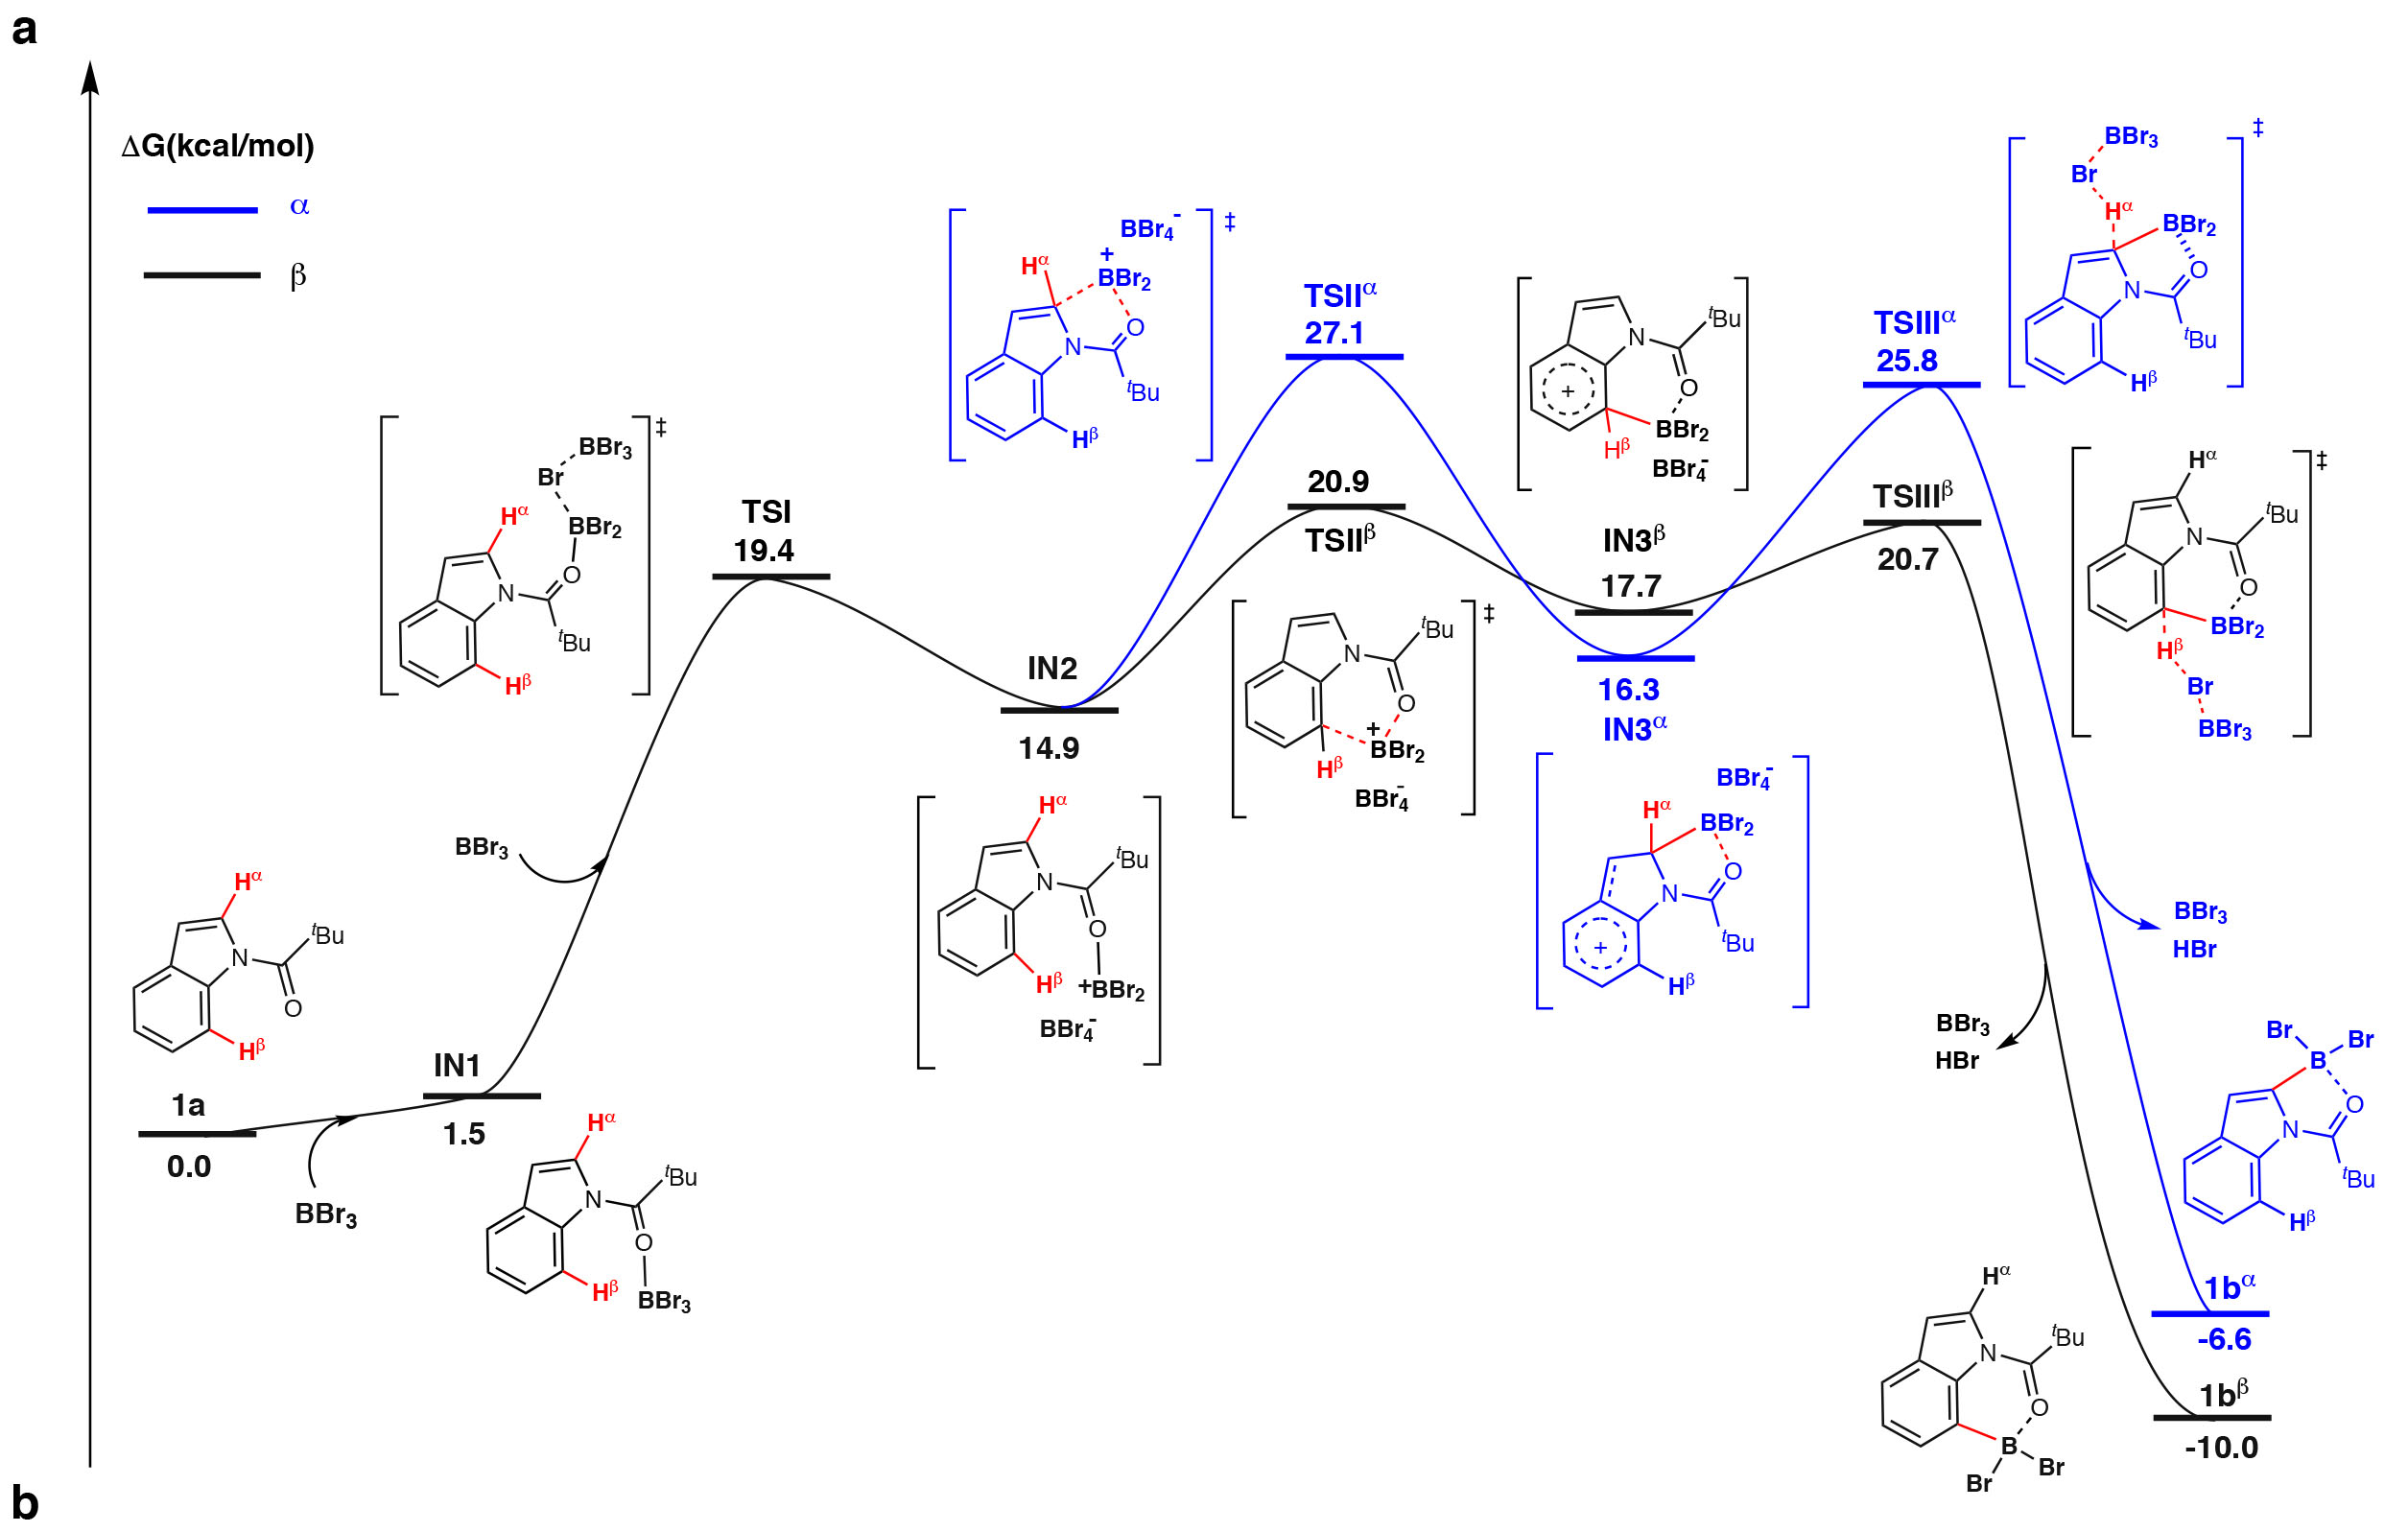
\includegraphics[width=0.93\linewidth]{metalfree-mech.jpg}
		%\caption{}
		\label{fig:metalfree-mech}
	\end{figure}
	
\end{frame}

\section{Annex}
\begin{frame}
	\frametitle{Acknowledgments}
	
	\begin{itemize}\setlength{\itemsep}{1.0cm}
		\item Prof. Jiao
		\item Associate Prof. Chen
		\item Authors of the brilliant works mentioned above
	\end{itemize}
\end{frame}
	\begin{frame}
		\frametitle{Annex}
		This slide and articles cited in the slide can be found here:\\[0.28cm] \small{ \textcolor{blue}{\url{https://github.com/Alexander-Qi/organoboron/releases/tag/\thisversion}}}
		
		
		
		\begin{figure}
			\centering
			Or Scan this QRcode:\\[0.35cm]
			
\includegraphics[width=0.2\linewidth]{fig/qrcode}
			\label{fig:qrcode}
		\end{figure}
		
	\end{frame}
\end{document}
